\section{Results, Dashboard, and Conclusion}

\subsection{Power BI Dashboard}

Power BI connects directly to the \texttt{wide\_streams} view in Snowflake using the Snowflake
ODBC connector.
Because all JOINs are pre-computed in the wide table, Power BI queries return results instantly
without requiring complex DAX measures or in-memory joins.

\begin{figure}[H]
  \centering
  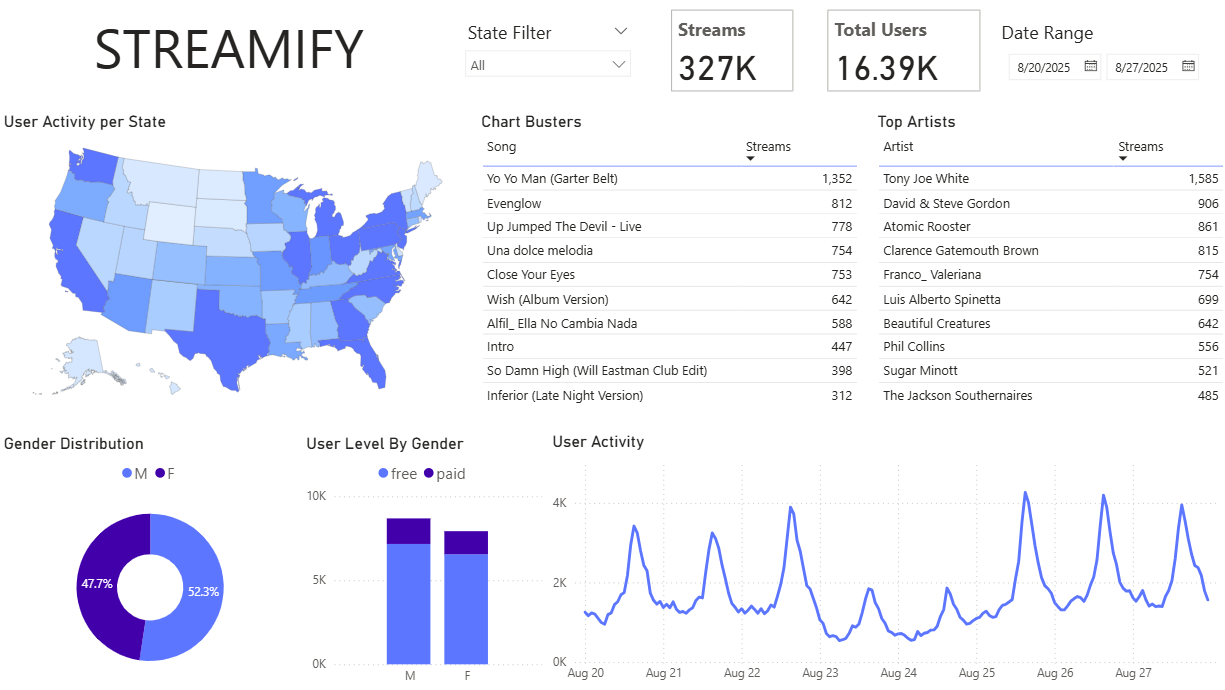
\includegraphics[width=0.92\textwidth]{../image/dashboard.png}
  \caption{Streamify Power BI dashboard: real-time music streaming analytics.}
  \label{fig:dashboard}
\end{figure}

Key metrics and visualisations on the dashboard:

\begin{itemize}
  \item \textbf{Top artists by play count} — bar chart showing the most-played artists over the selected date range.
  \item \textbf{Songs played over time} — time-series line chart with hourly granularity, revealing peak listening hours.
  \item \textbf{Geographic distribution} — map visual showing play counts by US state, derived from the \texttt{dim\_locations} dimension.
  \item \textbf{Subscription tier breakdown} — donut chart comparing free vs.\ paid listener proportions.
  \item \textbf{Session activity} — table showing active user sessions, authentication success rates, and average session duration.
\end{itemize}

\subsection{Pipeline Evaluation}

\begin{table}[H]
  \centering
  \caption{Streamify pipeline evaluation summary.}
  \label{tab:results}
  \begin{tabularx}{\textwidth}{lX}
    \toprule
    \textbf{Dimension}       & \textbf{Result} \\
    \midrule
    End-to-end latency       & TODO: measure from Eventsim event timestamp to Snowflake row visibility. \\
    Throughput               & TODO: events/second sustained under Eventsim default load. \\
    Fault tolerance          & Tested by killing a Flink TaskManager mid-run; job recovered from the latest checkpoint within seconds with no data loss. \\
    Exactly-once delivery    & Verified: no duplicate rows in Snowflake across multiple controlled restarts. \\
    Flink Web UI             & Job graph, checkpoint history, and back-pressure visualisation available at \texttt{http://localhost:8083}. \\
    dbt model freshness      & Star schema refreshed daily by Airflow; \texttt{wide\_streams} updated immediately after each dbt run. \\
    \bottomrule
  \end{tabularx}
\end{table}

\subsection{Conclusion and Future Work}

The Streamify project demonstrates a complete, production-pattern streaming pipeline built
on Apache Kafka and Apache Flink.
The migration from Spark Structured Streaming to PyFlink was transparent to all downstream
components (Snowflake, dbt, Airflow, Power BI) — confirming that the processing layer can be
swapped independently of the rest of the stack.

Key takeaways:
\begin{itemize}
  \item Kafka provides reliable, replay-capable event transport with zero changes required to producers or consumers when the processing engine changes.
  \item Flink's Table API and StatementSet pattern allow three independent Kafka→Snowflake pipelines to run as a single job with one shared checkpoint cycle.
  \item The ELT pattern (Flink loads raw data; dbt transforms inside Snowflake) cleanly separates streaming concerns from analytical modelling concerns.
\end{itemize}

Directions for future work:
\begin{itemize}
  \item \textbf{Flink CDC} — replace Eventsim with a Debezium CDC connector to stream changes from a real operational database.
  \item \textbf{Schema evolution} — integrate Confluent Schema Registry with Avro serialisation to handle backward-compatible schema changes.
  \item \textbf{Real-time ML} — embed a Flink ML model to compute real-time song recommendations and write them to a low-latency serving store (e.g.\ Redis).
  \item \textbf{Cloud deployment} — migrate from Docker Compose to a managed Flink service (e.g.\ Amazon Kinesis Data Analytics or Confluent Cloud) and a Managed Kafka cluster.
\end{itemize}
